\chapter{Généralité sur les drones convertible}
\minitoc
\label{chap:generalites}


\section{Micros drones convertibles}

    \subsection{Domaine de vol} 
    Tout l'intérêt d'un drone convertible réside dans sa capacité à décoller et atterrir verticalement, tout en conservant une bonne efficacité énergétique en vol d'avancement, grâce à une aile. Cette aile a l'avantage de générer de la portance, laquelle s'oppose au poids du drone et permet d'assurer sa sustentation. La contrepartie de la génération de la portance est la traînée qui s'oppose à l'avancement et doit être contrée par une force de traction générée par les hélices. Nous pouvons définir l'efficacité énergétique comme le ratio entre le temps de vol et l'énergie électrique nécessaire pour effectuer ce vol.
    
    Afin de souligner la prééminence de l'efficacité énergétique de ce modèle convertible, il convient de la comparer avec celle d'un drone quadrirotor qui assure sa sustentation uniquement grâce à des hélices (à l'instar d'un hélicoptère), et à celle d'un drone à voilure fixe.
    \begin{table}[ht]
        \centering
        \begin{tabular}{|c|c|c|c|c|}
            \hline
            Architecture & Vitesse $\SI{}{\meter\per\second}$  & Stationnaire & Temps de vol & Consommation\\
            \hline \hline
            Convertible & [0 - 30] & Possible & Quelques heures & Faible\\
            \hline
            Quadrirotor & [0 - 16] & Possible& Quelques minutes & Forte\\
            \hline
            Voilure fixe & [8 - 30] & Impossible & Plusieurs heures & Variable \\
            \hline
        \end{tabular}
        \caption{Comparaison des architectures de drone.}
    \end{table}

    Nous observons qu'un drone convertible possède un domaine de vol bien plus important qu'un drone à voilure fixe, lequel ne sera pas en mesure de voler à très basse vitesse, et qu'un quadrirotor, dont l'autonomie va être limitée par sa consommation.
    En alliant autonomie et vol stationnaire, le modèle convertible répond aux exigences des missions civiles et militaires.

    \subsection{Types d'architecture des drones convertibles}
    \label{sec:archConvertible}
    La conception structurelle et aérodynamique d'un drone est le facteur principal permettant des transitions stables et fluides. De plus, il est nécessaire d'optimiser l'architecture pour une mission, de manière à être le plus efficace. Au vu de la diversité des tâches à réaliser, un grand nombre de modèles ont été proposés, lesquels sont généralement catégorisables en trois classes : \textit{tiltrotor}, \textit{tailsitter}, \textit{tiltwing}. 
    En ce qu'il s'agit des prémices des convertibles, il parait opportun d'ajouter aux trois grandes catégories précédemment citées dans les états de l'art \cite{saeed_survey_2018,ducard_review_2021, review_2022}, la catégorie \textit{quadplanes}.

        \subsubsection*{\textit{Quadplanes}}
        Les \textit{quadplanes} résultent de la fusion d'un avion et d'un quadrirotor (comme visible sur la figure \ref{fig:quadplane}), ce qui permet un découplage de l'actionnement en fonction de la phase de vol. Le premier système de propulsion est composé de quatre hélices générant une force verticale permettant le contrôle lors des phases de décollage, d'atterrissage et stationnaire. Le second système de propulsion est composé d'une hélice propulsive supplémentaire afin de maintenir le vol d'avancement.

        \begin{figure}[ht!]
            \centering
                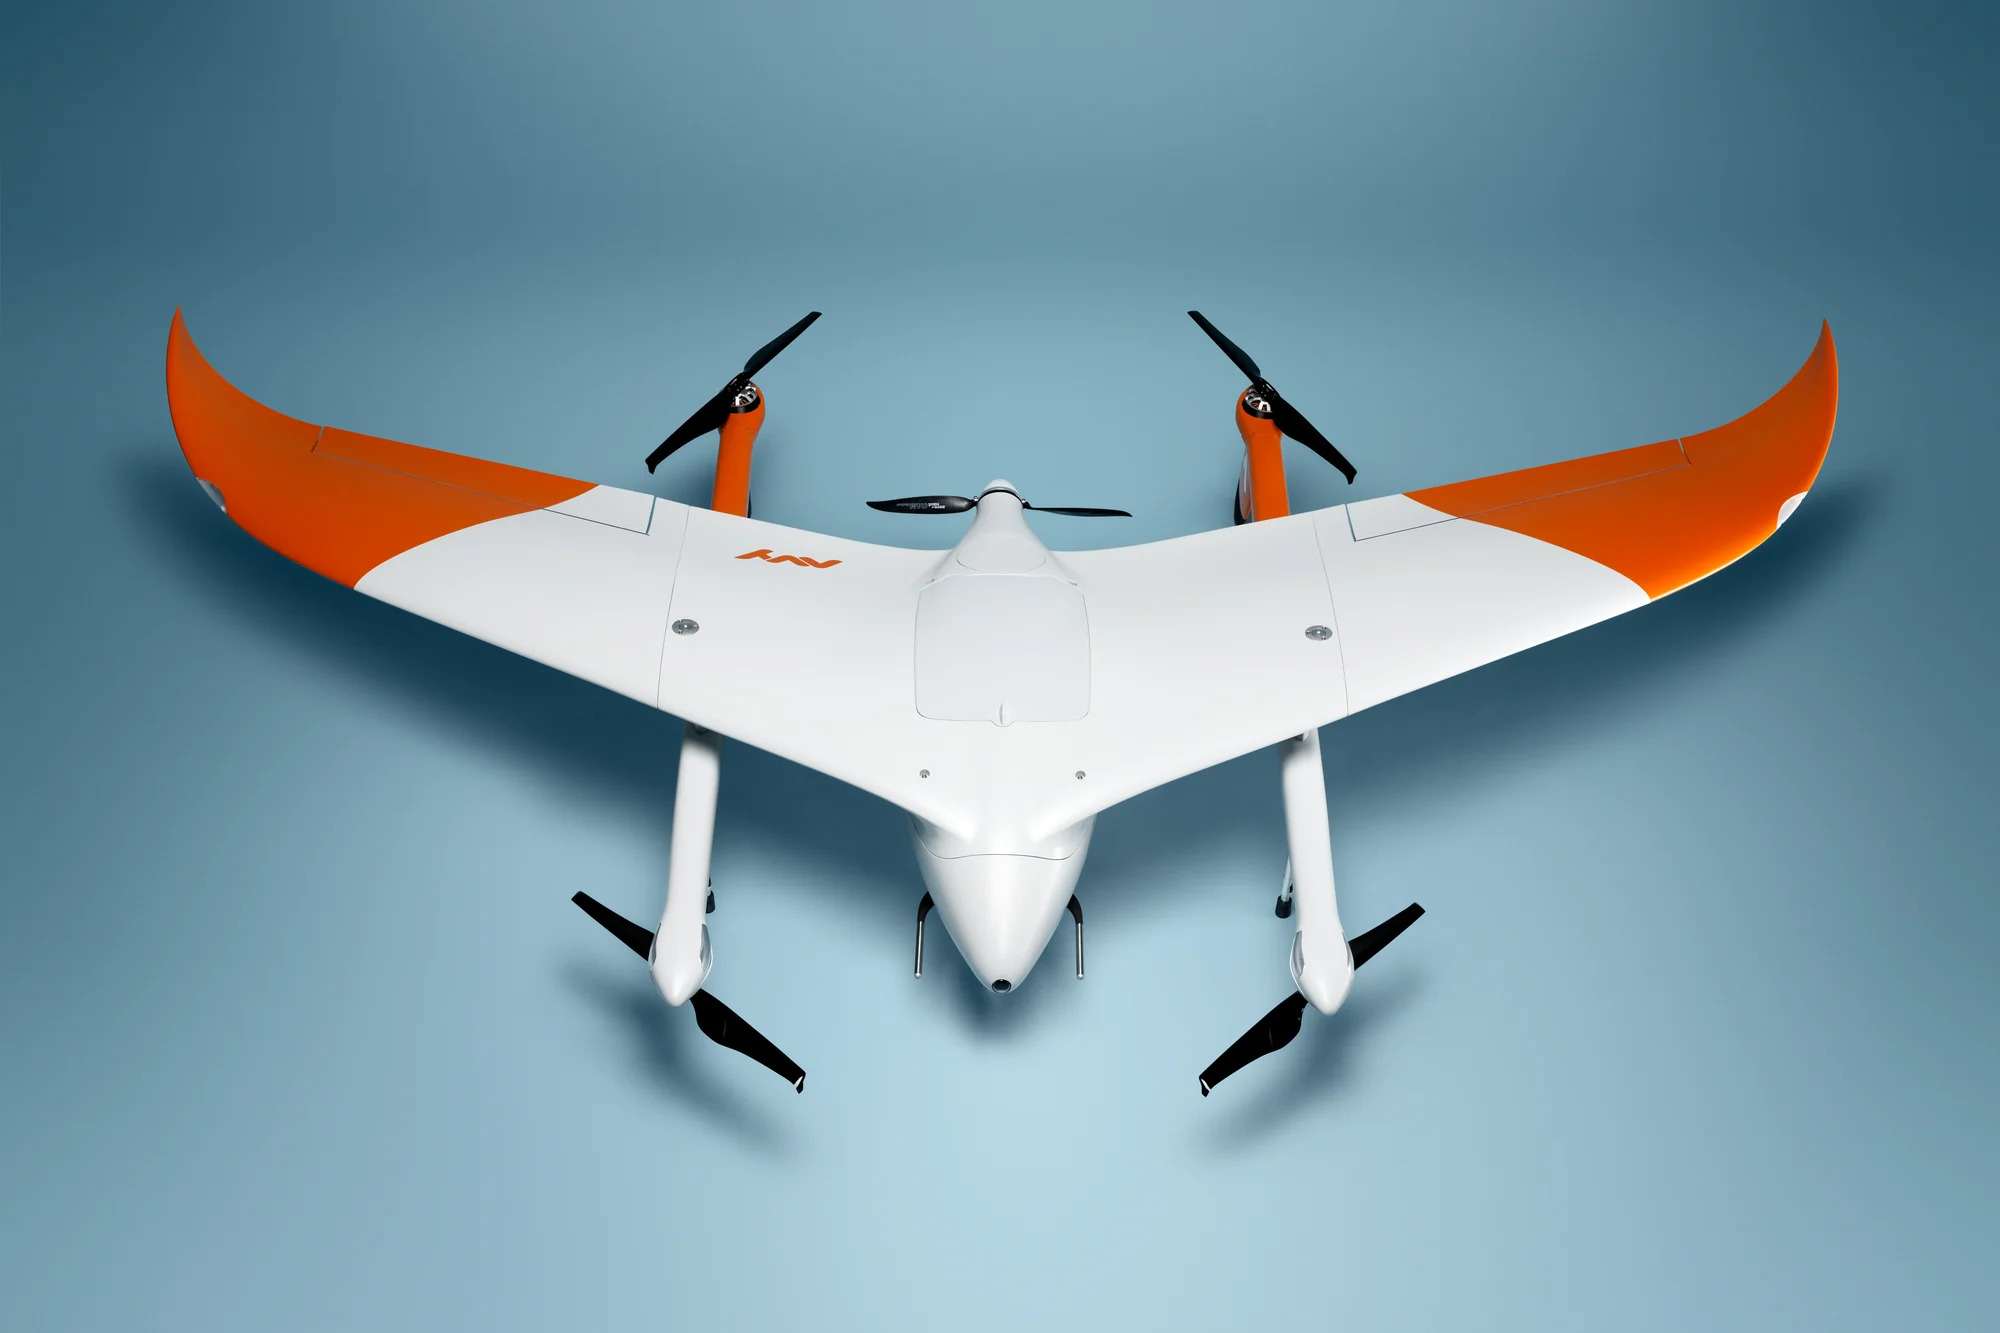
\includegraphics[width=0.6\columnwidth]{figures/Avy-Drone-quadplane.jpg}
                \caption{Structure \textit{quadplanes} proposée par \cite{Avy_2023}.}
                \label{fig:quadplane}
        \end{figure}
        

        L'avantage de ce type d'architecture est sa grande robustesse. Effectivement, aucune pièce en mouvement n'est nécessaire pour réaliser la transition, ce que réduit le risque de défaillance mécanique. Toutefois, l'inconvénient réside dans son manque d'efficacité. Lors d'un vol d'avancement, la portance sera générée par l'aile. Ainsi, il est possible de désactiver les rotors qui génèrent des perturbations aérodynamiques et des trainées parasites. Les axes des moteurs se retrouvent orthogonaux au flux d'air généré par le déplacement du drone, ce qui correspond au cas le plus défavorable en termes de trainée. De plus, la surcharge engendrée par l'emport de moteurs supplémentaires se traduit par une diminution de la charge utile transportable. 

        Pour ce qui est du contrôle, un atout indéniable est la séparation des actionnements en fonction des phases de vol. Ainsi, l'architecture de commande sera basée sur un mécanisme de commutation permettant de choisir la loi de commande appropriée sur un critère de vitesse air \cite{LiSongZhang2021, MathurAtkins2021, okulski2022small}. Ce critère est pertinent en ce qu'il est lié à la capacité de l'aile à générer de la portance induite par le flux d'air. Ainsi, à basse vitesse, le drone se stabilise avec l'actionnement quadrirotor et la loi de commande associée. Dans les vitesses plus importantes, la commutation de la loi permet de contrôler le drone en mode avion. Toutefois, le passage d'une loi à l'autre reste le point clé de la commande et demeure complexe et critique.

        \subsubsection*{\textit{Tiltrotor}}

        Les \textit{tiltrotors} nécessitent l'utilisation d'un actionneur dédié à la modification de l'orientation des moteurs. Les rotors sont montés sur des arbres basculants actionnés et la transition du vol stationnaire au vol d'avancement (ou inversement) s'effectue progressivement en fonction de l'inclinaison du rotor. Les deux configurations sont représentées sur la figure \ref{fig:tiltrotor}. Ainsi, l'angle entre le souffle des hélices et l'aile peut être ajusté à chaque instant \cite{9836063, du2024numerical, nie2024hierarchical, schlatter2024longitudinal}. Cet angle joue un rôle important dans le contrôle des forces et des moments aérodynamiques : sa maîtrise permet, non seulement, de mieux gérer les performances aérodynamiques du vol lors des transitions, mais aussi la stabilité du système sur l'ensemble du domaine de vol. 
        Malgré le fait que les \textit{tiltrotor} embarquent un actionneur uniquement dédié à la transition, ce qui augmente la masse du drone, cette architecture est intéressante car elle permet d'utiliser les mêmes actionneurs pour assurer la sustentation en stationnaire et pour générer la traction en mode avion.
        \begin{figure}[ht!]
            \centering
            \resizebox{.9\textwidth}{!}{%
            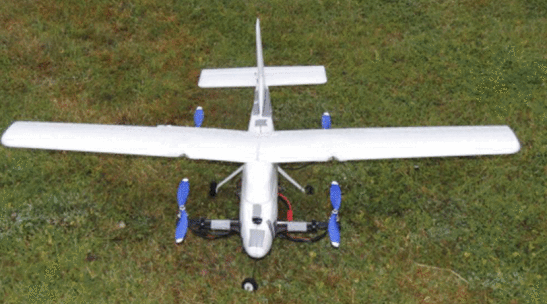
\includegraphics[height=3cm]{figures/tiltrotorhover.png}
            \quad
            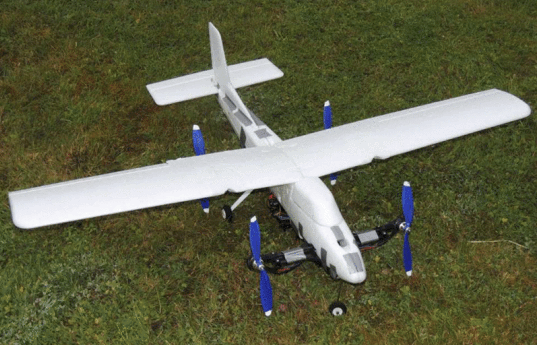
\includegraphics[height=3cm]{figures/tiltrotorforward.png}
            }
            \caption{Structure \textit{Tiltrotor}  proposée par \cite{7040348}, dans deux configurations, vol stationnaire et d'avancement.}
            \label{fig:tiltrotor}
        \end{figure}


        

        \subsubsection*{\textit{Tailsitter}}
        Contrairement aux \textit{tiltrotors} qui se posent sur le fuselage de l'avion (figure \ref{fig:tiltrotor}), les \textit{tailsitter} se posent à la verticale (voir figure centrale \ref{fig:tailsitter}). Durant la transition du mode stationnaire au vol d'avancement, la structure entière bascule vers l'avant, modifiant ainsi l'angle d'incidence de la voilure \cite{RobinRaffaello2017, VerlingWeibelSiegwart2016,smeurINDITail, ChiappinelliNahon2018, tal2022global}. Selon la configuration du \textit{tailsitter}, la transition peut être réalisée soit par la génération du moment aérodynamique créé par les élevons, soit par le couple créé par le système de propulsion. Pendant le vol d'avancement, en position horizontale, le \textit{tailsitter} vole comme un avion conventionnel sans dérive. En utilisant des techniques aérodynamiques classiques, les concepteurs peuvent optimiser le profil de l'aile du \textit{tailsitter} pour le rendre plus endurant afin de réduire la consommation d'énergie. Grâce à ce processus d'optimisation aérodynamique, le \textit{tailsitter} peut effectuer des missions de vol de plus d'une heure.

        \begin{figure}[ht!]
            \centering
            \resizebox{.9\textwidth}{!}{%
            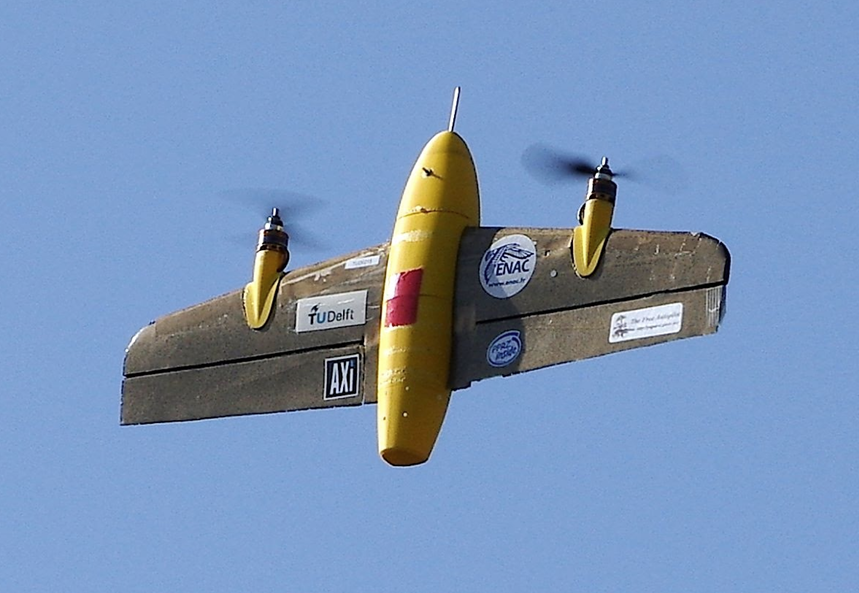
\includegraphics[height=3cm]{figures/cyclone.png}
            \quad
            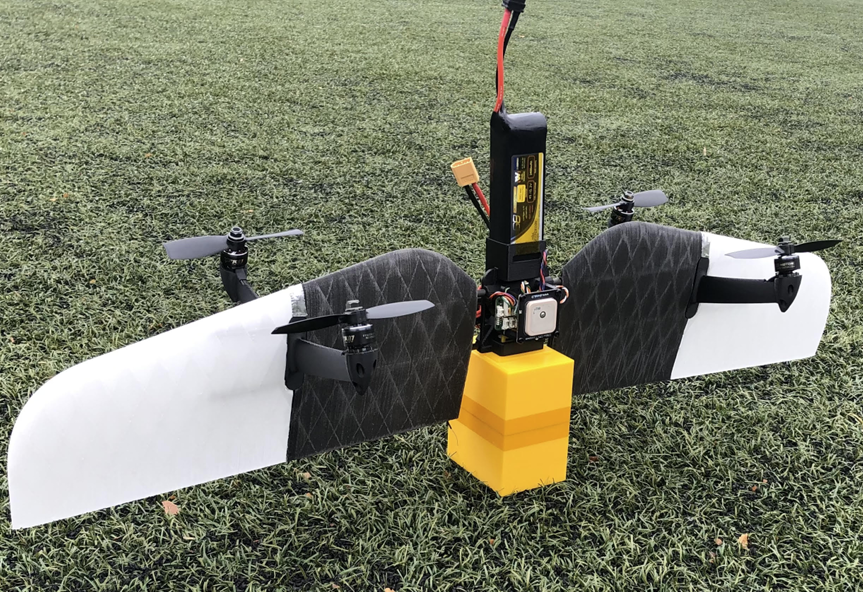
\includegraphics[height=3cm]{figures/falcon.png}
            \quad
            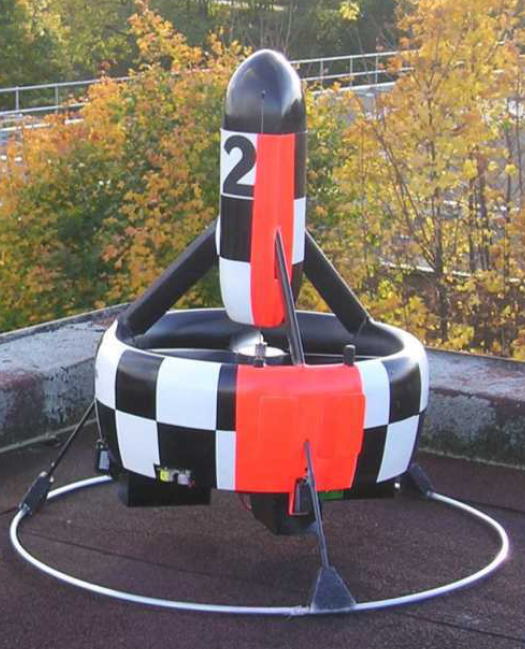
\includegraphics[height=3cm]{figures/HoverEye.png}
            }
            \caption{Structure \textit{tiltrotor}  proposée par \cite{smeurINDITail,fernandez:hal-04612206,pflimlin:tel-00132352}.}
            \label{fig:tailsitter}
        \end{figure}
        
 
        Ce modèle semble être la configuration la plus intéressante énergétiquement, car il utilise les mêmes actionneurs dans tout le domaine de vol. Ainsi, aucune masse superflue n'est embarquée.

    
        \subsubsection*{\textit{Tiltwing}} 
        La particularité des \textit{tiltwings} réside dans le fait que les rotors sont inclinés en même temps que les ailes (voir figure \ref{fig:tiltwing}). Un actionneur supplémentaire et puissant est donc nécessaire pour surmonter le couple de l'aile afin de la positionner dans l'orientation souhaitée \cite{holsten2011design, rohr2019attitude, ccetinsoy2012design}. La commande de cet actionneur doit être prise en compte lors de la conception des lois de commande. Pendant le décollage, l'atterrissage et les vols stationnaires, les ailes doivent être positionnées vers le haut afin de produire une force de poussée opposée au vecteur gravité. Dans ces phases de vol, lorsque les ailes sont orientées vers le haut, l'aéronef est plus vulnérable au vent et les lois de commande doivent rejeter ces perturbations. Dans la littérature, il existe plusieurs configurations d'ailes basculantes et différentes approches de contrôle conçues pour stabiliser leur dynamique de vol.
        \begin{figure}[ht!]
            \centering
            \resizebox{.9\textwidth}{!}{%
            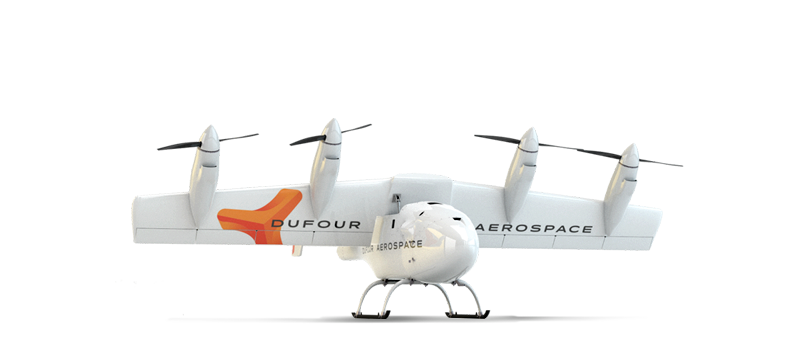
\includegraphics[height=3cm]{figures/tiltwing_aero2.png}
            \quad
            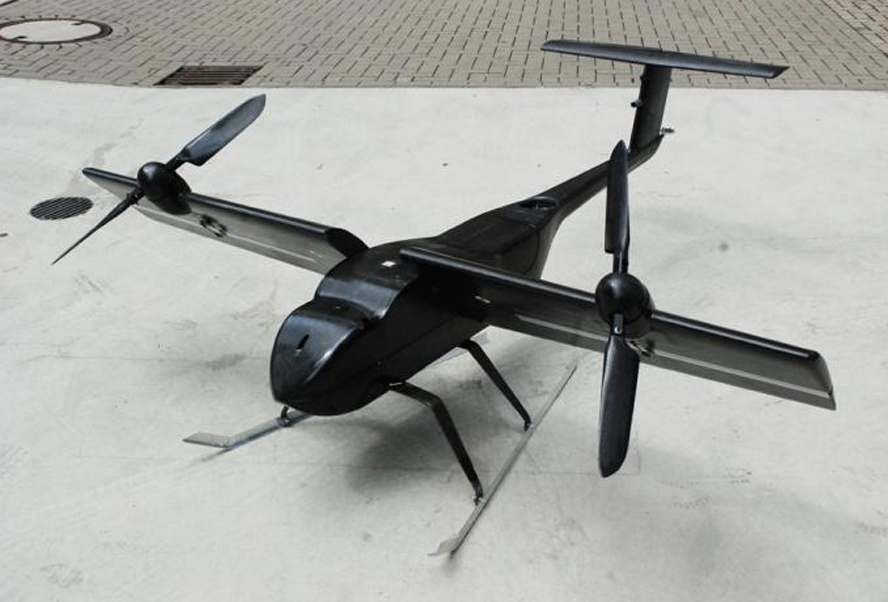
\includegraphics[height=3cm]{figures/avigle_tiltwing.png}
            }
            \caption{Structure \textit{tiltwings}  proposée par \cite{Aero2_2024, Ostermann2012ControlCO}.}
            \label{fig:tiltwing}
        \end{figure}

        Par ailleurs, les \textit{freewing} sont une gamme en cours de développement à l'intérieur de l'architecture des \textit{tiltwing}. Ils sont actionnés comme des \textit{tiltwing}, excepté au niveau de l'axe de rotation entre l'aile et le fuselage. Cette rotation est laissée libre, ce degré de liberté permettant à l'aile de changer librement son incidence. Il en résulte un gain de masse car il est possible de supprimer l'actionneur puissant et lourd nécessaire à la rotation de l'aile. De plus, l'aile étant libre de s'orienter, les turbulences ont un impact plus faible sur la structure, ce qui rend les vols plus stables \cite{freewing2012, Johnson2021, Johnson2023}. 


\section{Propriétés des \textit{tailsitters} et des \textit{freewings}}
    D'un point de vue mécanique, les \textit{tailsitters} et les \textit{freewings} sont caractérisés comme des systèmes sous-actionnés avec une dynamique fortement couplée. Ces caractéristiques mécaniques rendent le processus de modélisation et d'identification difficile. Cela peut s'expliquer par le fait que, pour ce type de système, une entrée de commande donnée agit simultanément sur différentes dynamiques. Ainsi, l'identification de l'influence d'une entrée de commande donnée sur une dynamique particulière reste un processus important qui nécessite plus d'attention.
    \subsection{Actionnement}
    Dans ces deux architectures, il est courant de trouver des actionneurs basés sur des effets aérodynamiques. Ces actionneurs ont l'avantage d'être peu consommateurs en énergie. Ils sont mus par des servomoteurs qui consomment peu d'électricité proportionnellement au couple qu'ils génèrent. Dans le cas des ailes volantes, les surfaces aérodynamiques sont souvent placées sur la partie arrière des ailes et peuvent être utilisées symétriquement à l'instar de volets, ou anti-symétriquement comme des ailerons. 
    Dans les phases de décollage, de vol stationnaire ou d'atterrissage, la plateforme est maintenue en vol par les hélices : il est donc nécessaire de dimensionner les groupes moteurs-hélices pour qu'ils puissent générer assez de force. En fonction des configurations, les moments peuvent être obtenus par des différentiels sur l'utilisation des moteurs ou bien par des surfaces aérodynamiques. Dans le cas de surfaces soufflées par le flux d'air des hélices, il existe un couplage des actionneurs qui complexifie la modélisation et le contrôle de ces architectures.

    \todo{Sous actionnement}

    \begin{definition}[Sous-actionnement]
        Considérons la dynamique d'un système décrite par l'équation différentielle du second ordre :
        \begin{align*}
            \ddot{\boldsymbol{q}} = f_1(\boldsymbol{q}, \dot{\boldsymbol{q}}, t) + f_2(\boldsymbol{q}, \dot{\boldsymbol{q}}, t) \boldsymbol{u}
        \end{align*}
        où $\boldsymbol{q} \in \real^{n}$ est le vecteur d'état de dimension $n$, $\boldsymbol{u} \in \real^{m}$ est le vecteur de commande de dimension $m$ et $t$ le temps. 

        Lorsque le rang de $f_2$ est inférieur à la dimension du vecteur $\boldsymbol{q}$, on dit que le système est sous-actionné :
        \begin{align*}
            rank[f_2(\boldsymbol{q}, \dot{\boldsymbol{q}}, t)] < dim[\boldsymbol{q}]
        \end{align*}
    \end{definition}

    \subsection{Aérodynamique}

    Lors d'un vol d'avancement, les \textit{tailsitters} et les \textit{freewings} assurent le maintien du vol en palier, en générant une force de portance grâce à leur surface alaire. Cette portance, qui s'opposant au poids, permet de maintenir une trajectoire. La force de trainée engendrée par l'aile et le fuselage est compensée par la composante horizontale de la poussée. En vol stationnaire, le poids est compensé par la traction de l'hélice. La relation d'équilibre est plus complexe lorsque nous évaluons l'ensemble des points d'équilibre lors de la transition d'un mode à l'autre. La transition équilibrée est assurée par le mélange correct des forces aérodynamiques et de propulsion.

    Les interactions aérodynamiques entre l'hélice et la surface de l'aile sont connues pour être complexes et difficiles à modéliser. La vitesse induite par le souffle de l'hélice entraîne une variation locale de l'angle d'attaque et des variations de pression dynamique au niveau des sections d'aile immergées, d'où une distribution différente de la portance. L'analyse de l'interaction entre l'hélice, l'aile et les élevons doit permettre d'obtenir de bonnes caractéristiques de vol et de tirer profit des combinaisons.

    \begin{figure}[ht!]
        \centering
            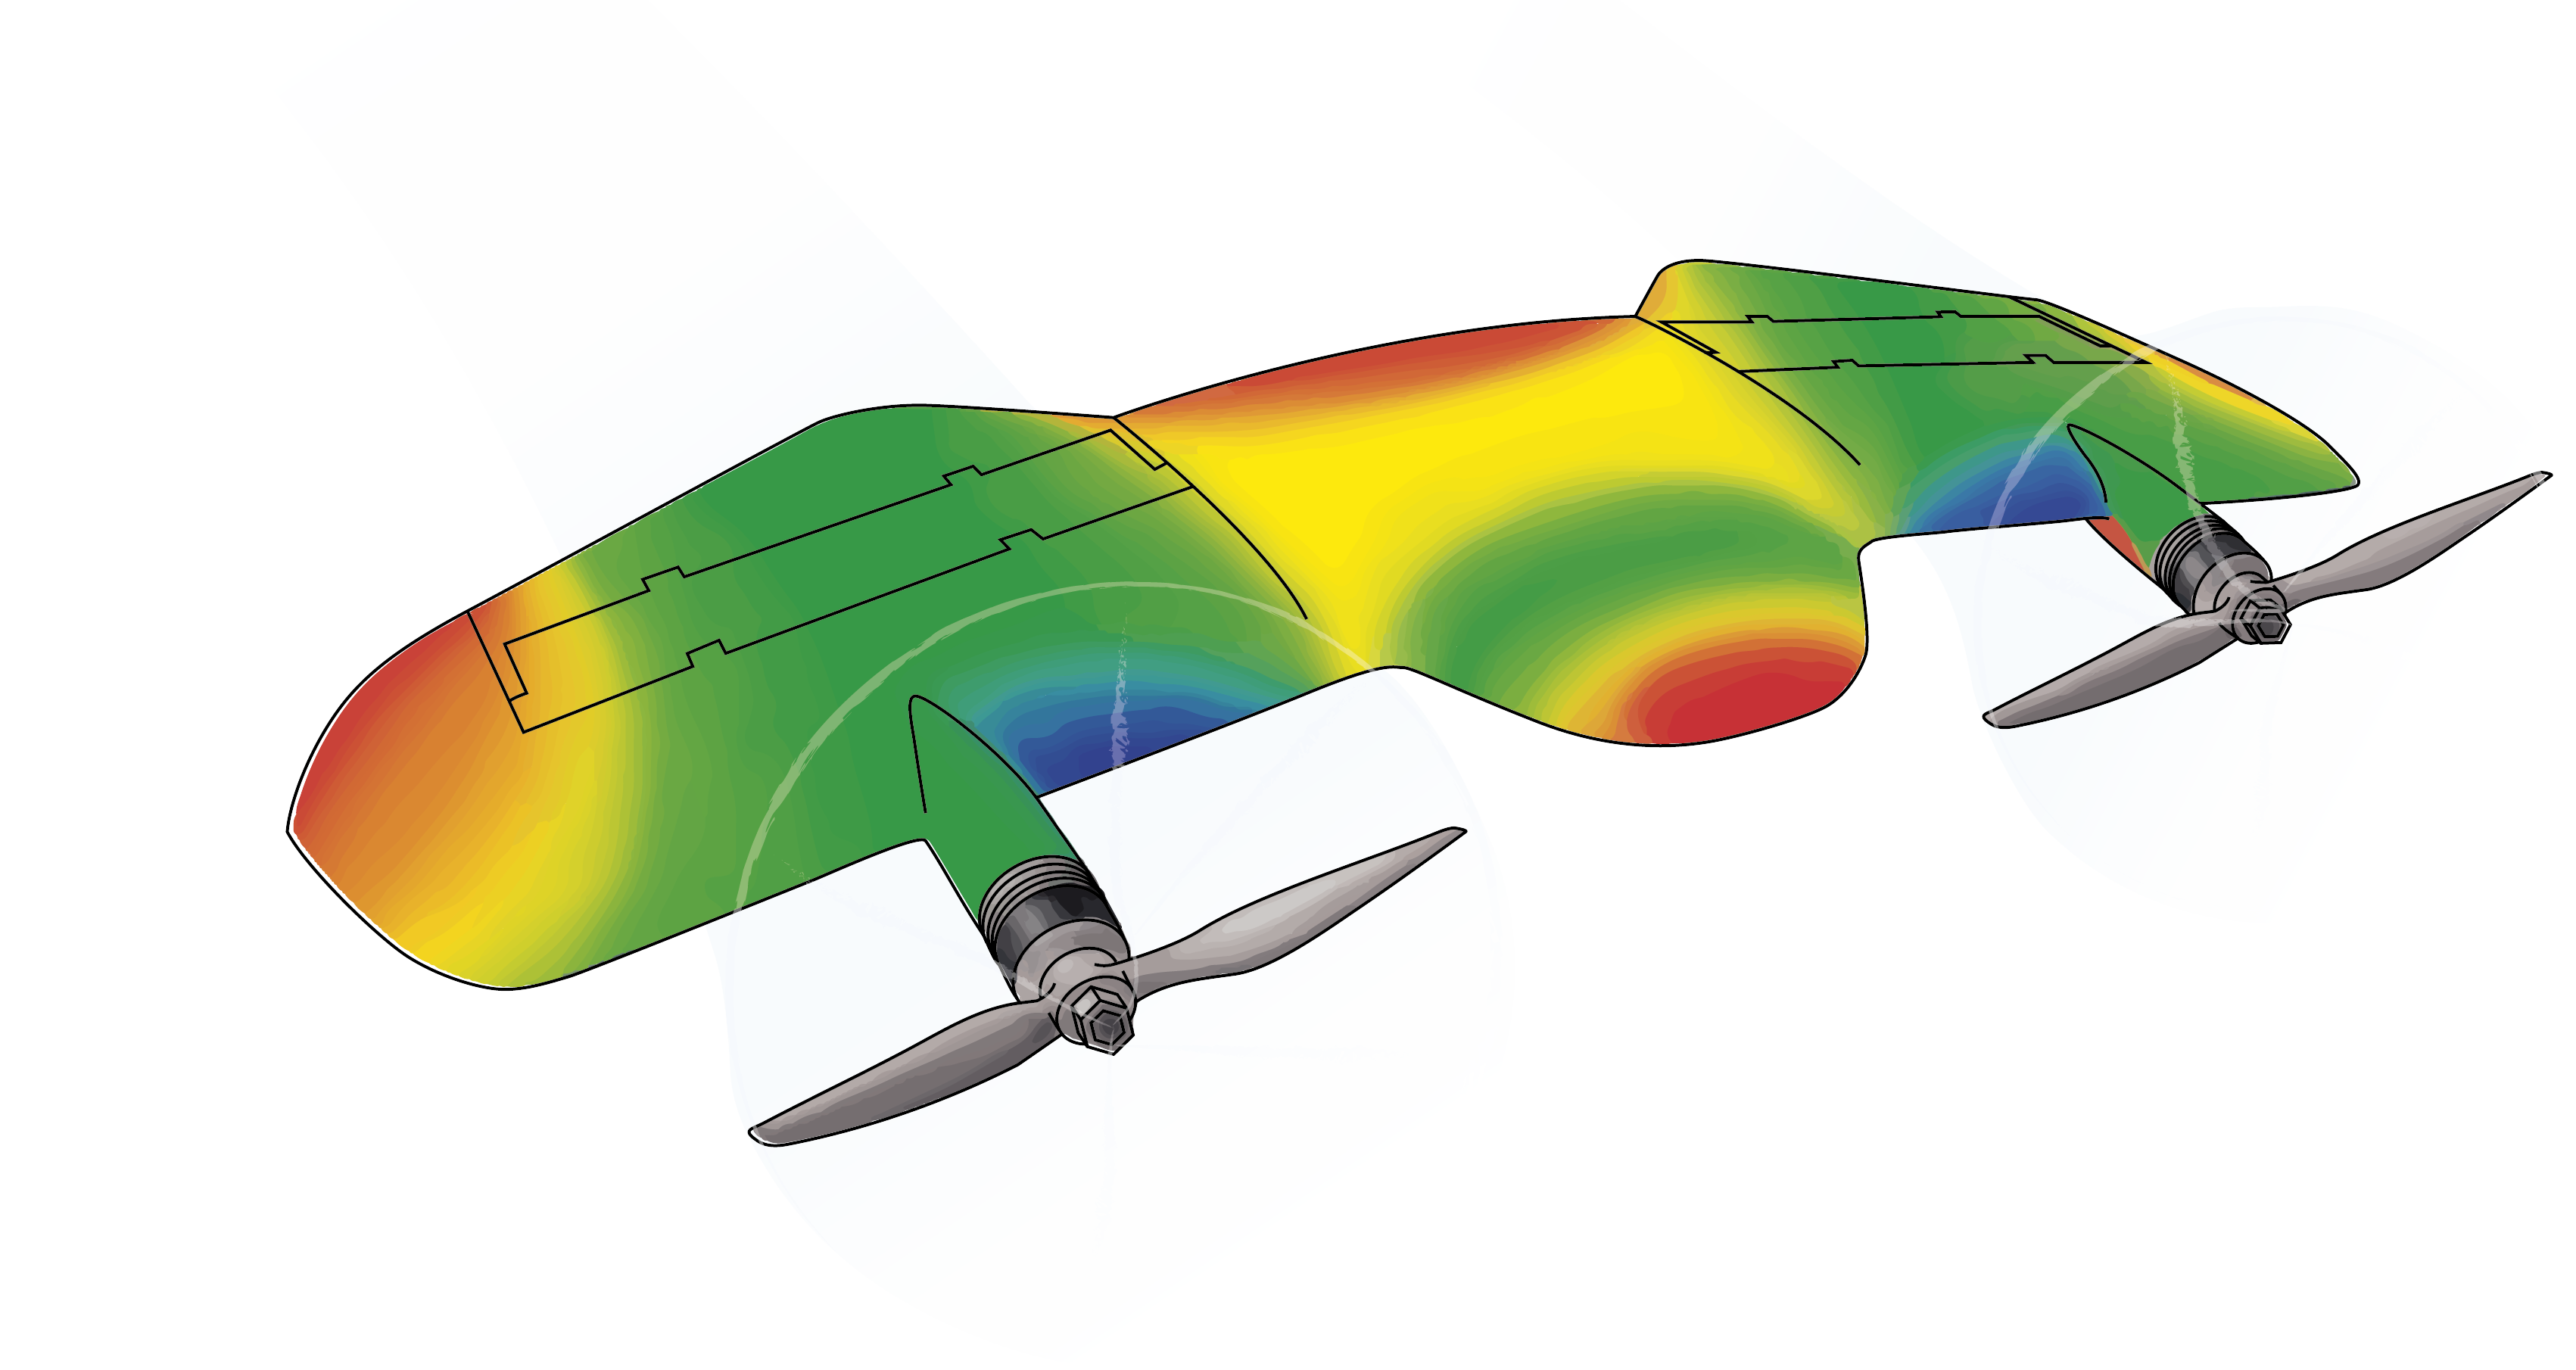
\includegraphics[width=0.6\columnwidth]{figures/Darko-air-pressure.png}
            \caption{Représentation de la pression dynamique sur la voilure de DarkO lors d'un vol d'avancement.}
            \label{fig:darkoAirPress}
    \end{figure}

     L'identification de ces effets aérodynamiques nécessite, pour chaque point de vol, les informations de l'air environnant, les valeurs des entrées de commande et les mesures des forces et moments aérodynamiques agissant sur le système. Le moyen le plus précis et le plus fiable d'identifier les phénomènes aérodynamiques est probablement de mener des campagnes en soufflerie, lesquelles sont particulièrement chronophages et coûteuses.


\section{Modélisations}
Dans le cas des drones convertible basculant, le modèle aérodynamique doit être correct dans les phases de transition. Cela nécessite l'extension de l'aérodynamique classique (faible incidence) à un angle d'attaque élevé et à un fonctionnement à faible vitesse. En outre, l'effet du souffle de l'hélice sur les profils aérodynamiques du véhicule doit être compris et pris en compte dans le modèle du système. Par exemple, les travaux de \cite{9444145} sur un \textit{tiltwing} identifient les zones d'interaction entre l'hélice et l'aile. Ils séparent clairement la génération de force et de couple lesquelles sont obtenues par la partir soufflée et non-soufflée de l'aile.

Des fonctions non linéaires continues décrivant les coefficients de portance et de traînée aérodynamiques sur toute la plage de l'angle d'attaque pour les  \textit{tiltrotors} ont été dérivées dans \cite{6981467} et pour les \textit{tiltwing} dans \cite{lustosaHal-03035938,Lustosa2017LaP}.

Il existe de nombreuses conceptions possibles pour un drone convertible. Bien que tous les modèles aient une structure commune, il existe des différences majeures dans la formulation réelle des termes de force et de couple. Celles-ci dépendent de la disposition des moteurs ou des hélices, de l'existence ou non de surfaces de contrôle aérodynamiques et de la forme du véhicule.

Un modèle précis est nécessaire pour les conceptions classiques de contrôle basées sur un modèle et en particulier pour les approches d'inversion dynamique ou de contrôle prédictif de modèle. Cependant, une modélisation précise va nécessiter une campagne d'identification approfondie en soufflerie ou un vol en environnement contraint. Il se peut également que la complexité du modèle ne permette pas une utilisation directe dans le contrôle à cause de limitation matérielle des calculateurs embarqué.


Dans notre cas, nous nous sommes intéressés à l'impact du vent sur les architectures mentionnées précédemment. Il est donc nécessaire de modéliser le vent. Dans le cas de vent constant ou de cisaillement de vent, un modèle à échelons semble tout à fait approprié pour représenter le changement brusque de vitesse de vent. 
Pour les rafales, nous utiliserons plusieurs modèles, tel que le modèle "Chapeau mexicain" ou les "ondelettes de Morlet".

La fonction définissant le chapeau mexicain est :
\begin{align}
    \Psi_{mex}(t)= w_{m} - \frac{A_g}{2} \left(1-\cos(2 \pi f_g (t-t_{0,mex}))\right)\sin(3 \pi f_g (t-{0,mex}))
\end{align}
et la fonction ondelettes de Morlet est défini par :
\begin{align}
    \Psi_{mor}(t)=  w_{m} + A_g \exp(-(t+t_{0,mor})) \cos(5*(t-t_{0,mor}))
\end{align}
où $w_{m}$ est le vent moyen sans perturbation, $t_{0,mex}$ représente l'instant de début de perturbation et $t_{0,mor}$ l'instant où la perturbation est maximale, $A_g$ est l'intensité maximale de la perturbation et  $f_g$ est la fréquence de la perturbation. Les tracés de la figure \ref{fig:mexhat} montrent la représentation temporelle des deux fonctions pour les valeurs $w_{m} = \SI{1}{\meter\per\second}$, $t_{0,mex} = \SI{2}{\second}$,  $t_{0,mor} = \SI{5}{\second}$, $A_g = \SI{1}{\meter\per\second}$ et $f_g = \SI{0.8}{\radian\per\second}$.


\begin{figure}[ht!]
    \centerline{
    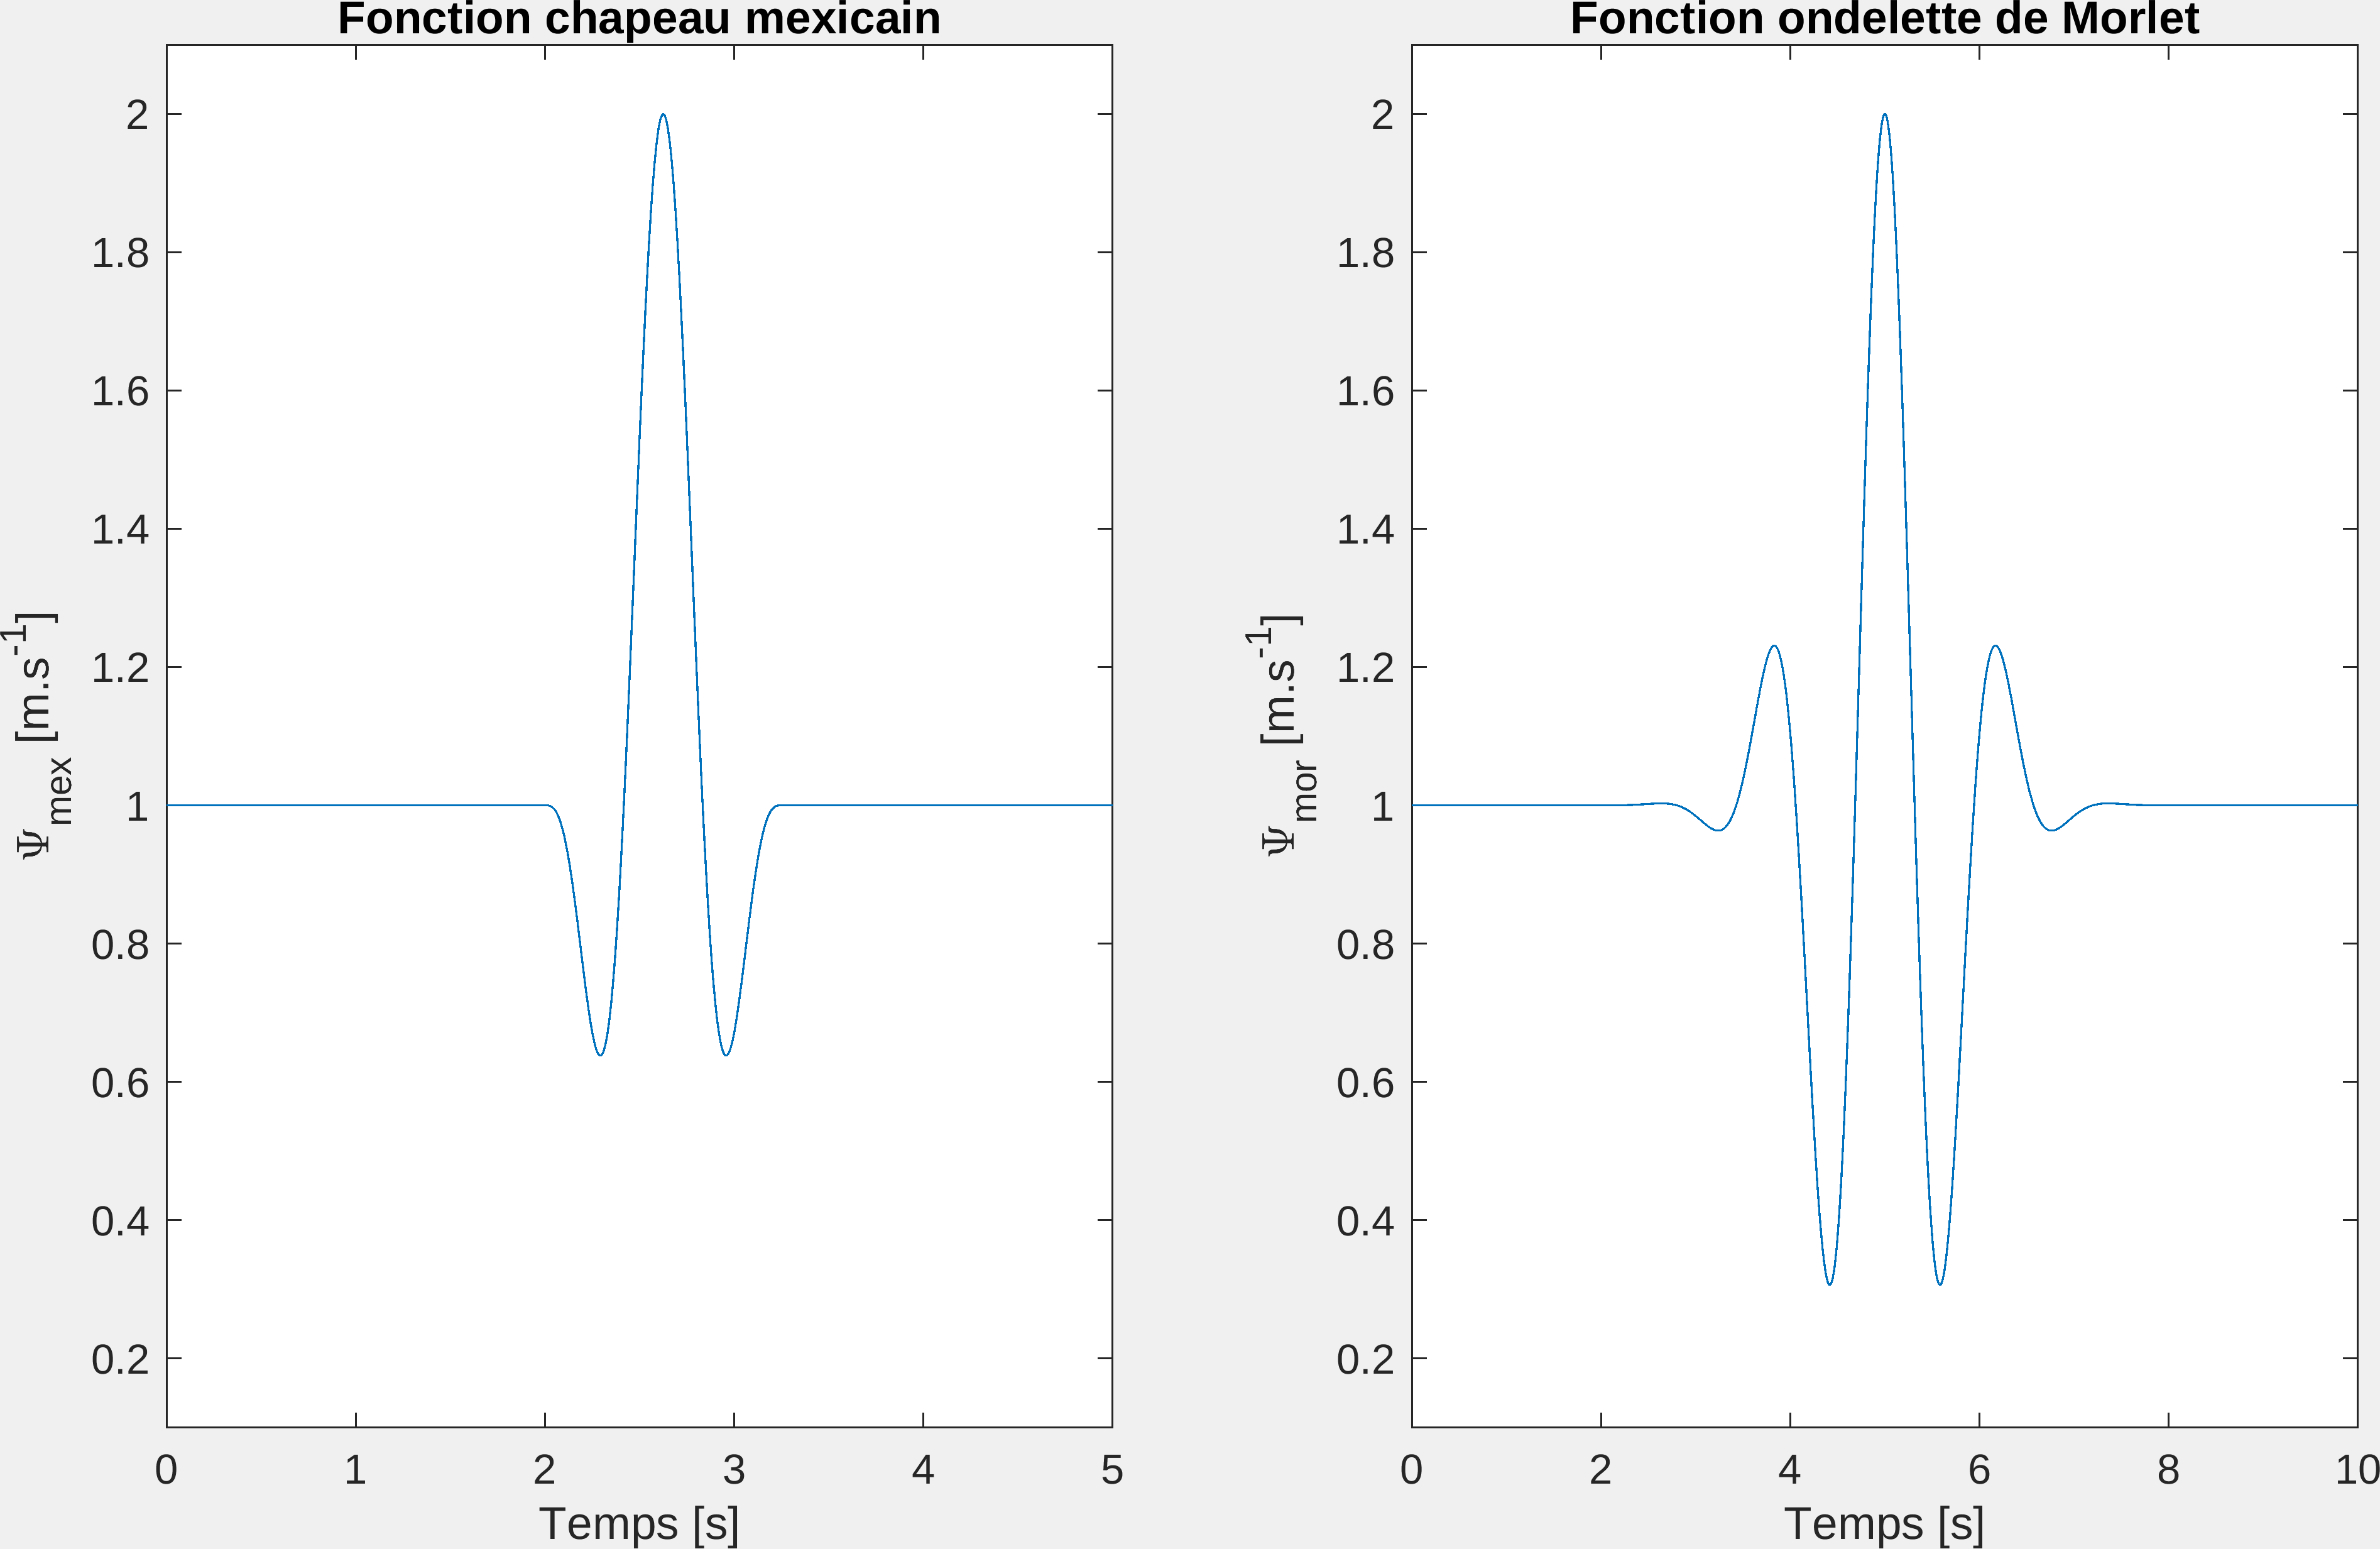
\includegraphics[trim=0cm 0cm 0cm 0cm,clip,width=0.9\columnwidth]{figures/mex_hat_morlet.png}}
    \caption{Représentation temporelle des modèles de perturbations de vent.}
    \label{fig:mexhat}
\end{figure}


% Le modèle de Dryden est défini :
% \begin{subequations}
%     \begin{align}
%         \Phi _{u_{g}}(\Omega )& =\sigma _{u}^{2}{\frac {2L_{u}}{\pi }}{\frac {1}{1+(L_{u}\Omega )^{2}}}\\
%         \Phi _{v_{g}}(\Omega )& =\sigma _{v}^{2}{\frac {2L_{v}}{\pi }}{\frac {1+12(L_{v}\Omega )^{2}}{\left(1+4(L_{v}\Omega )^{2}\right)^{2}}}\\
%         \Phi _{w_{g}}(\Omega )& =\sigma _{w}^{2}{\frac {2L_{w}}{\pi }}{\frac {1+12(L_{w}\Omega )^{2}}{\left(1+4(L_{w}\Omega )^{2}\right)^{2}}}
%     \end{align}
% \end{subequations}
% \todo{explication}
% Le modèle de von Kármán :
% \begin{subequations}
%     \begin{align}
%         \Phi _{u_{g}}(\Omega )& =\sigma _{u}^{2}{\frac {2L_{u}}{\pi }}{\frac {1}{\left(1+(1.339L_{u}\Omega )^{2}\right)^{\frac {5}{6}}}}\\
%         \Phi _{v_{g}}(\Omega )& =\sigma _{v}^{2}{\frac {2L_{v}}{\pi }}{\frac {1+{\frac {8}{3}}(2.678L_{v}\Omega )^{2}}{\left(1+(2.678L_{v}\Omega )^{2}\right)^{\frac {11}{6}}}}\\
%         \Phi _{w_{g}}(\Omega )& =\sigma _{w}^{2}{\frac {2L_{w}}{\pi }}{\frac {1+{\frac {8}{3}}(2.678L_{w}\Omega )^{2}}{\left(1+(2.678L_{w}\Omega )^{2}\right)^{\frac {11}{6}}}}
%     \end{align}
% \end{subequations}



\section{Actionnements}

\begin{figure}[ht!]
    \centerline{
    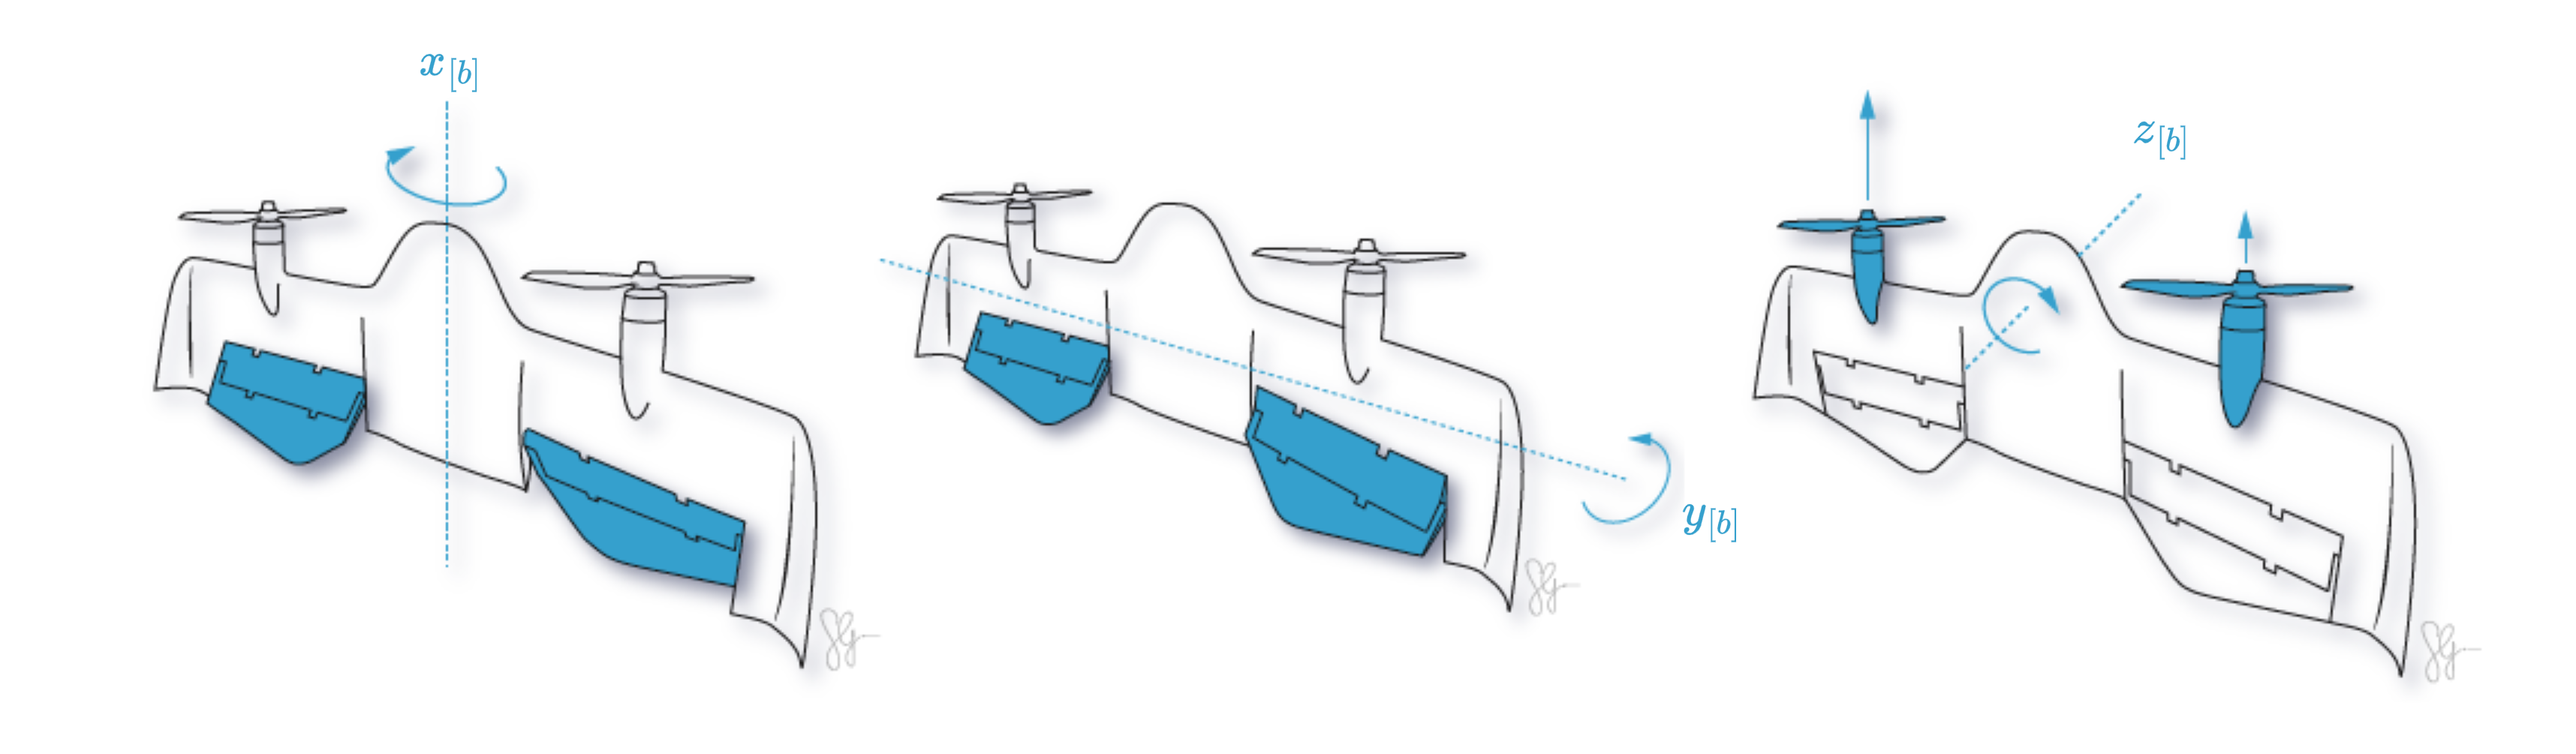
\includegraphics[trim=0cm 0cm 0cm 0cm,clip,width=1\columnwidth]{figures/actionnement.png}}
    \caption{Actionneurs d'un \text{tailsitter} et leurs actions sur les axes principaux.}
    \label{fig:actionDarko}
\end{figure}

La figure \ref{fig:actionDarko} illustre les effets des actionneurs sur la dynamique de l'attitude des \textit{tailsitters}. La rotation autours de l'axe $x_{\text{b}}$ peut être contrôlé par des braquages de volets asymétriques, l'angle de tangage (axe $y_{\text{b}}$) par des braquages de volets symétriques et la rotation autour de l'axe $z_{\text{b}}$ est contrôlée par un dispositif de poussée différentielle, ce qui permet d'obtenir un angle de tangage plus élevé. La rotation autour de l'axe de lacet est contrôlée par une configuration de poussée différentielle, qui crée un couple temporaire non nul autour de son axe. Le dispositif de poussée différentielle engendre une différence entre les rotations de l'hélice gauche et de l'hélice droite, et modifie ainsi la vitesse de rotation de l'avion et donc le comportement aérodynamique autour des volets.


\section{Architectures de commande de vol}


Une approche en cascade est une méthode couramment utilisée dans le cadre de la commande de drone. Cette approche est basée sur l'imbrication de boucle de  commande illustrée sur la Figure \ref{fig:schemahiera}. 
Cette architecture s'appuyer sur la séparation des dynamiques d'un drone sous actionné. Effectivement, comme le drone est obligé de modifier son orientation pour changer de position, le schéma de contrôle prend en compte cette spécificité. Ainsi la boucle interne est réglé pour avoir un temps de réponse faible vis-à-vis des autres lois. Cette boucle interne stabilise l'attitude du drone $att_{m}$ en la faisant converger vers l'attitude de consigne $att_{c}$. Cette attitude de consigne est le résultat de la boucle de vitesse qui fait converger la vitesse du drone $vel_{m}$ vers la vitesse de consigne $vel_{c}$. La vitesse de consigne est la résultante de la boucle de position qui fait converge la position du drone $pos_{m}$ vers la position de consigne défini par le pilote $pos_{c}$.
\begin{figure}[ht!]
    \centerline{
    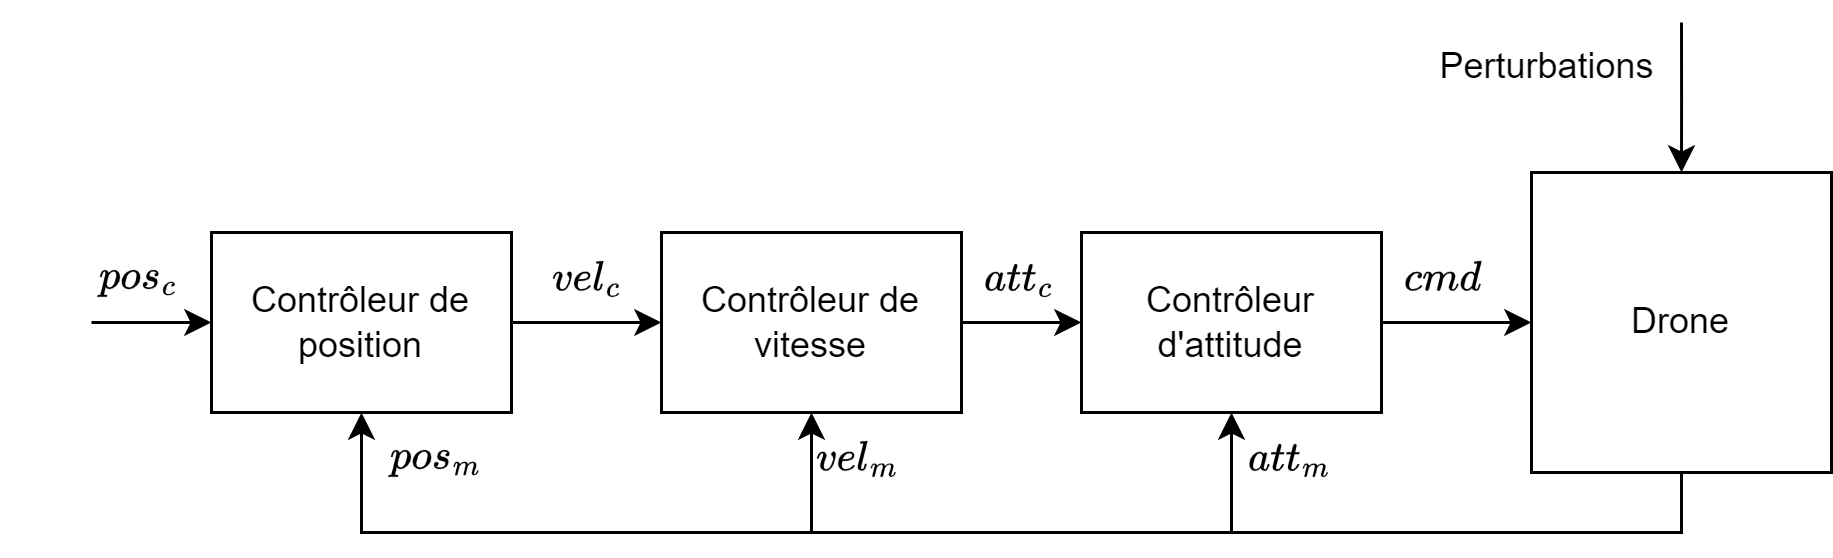
\includegraphics[trim=0cm 0cm 0cm 0cm,clip,width=0.8\columnwidth]{figures/controlhierachique.png}}
    \caption{Architecture classique de contrôle hiérarchique pour les drones.}
    \label{fig:schemahiera}
\end{figure}


\section{Méthodes de commande}
\begin{figure}[ht!]
    \centerline{
    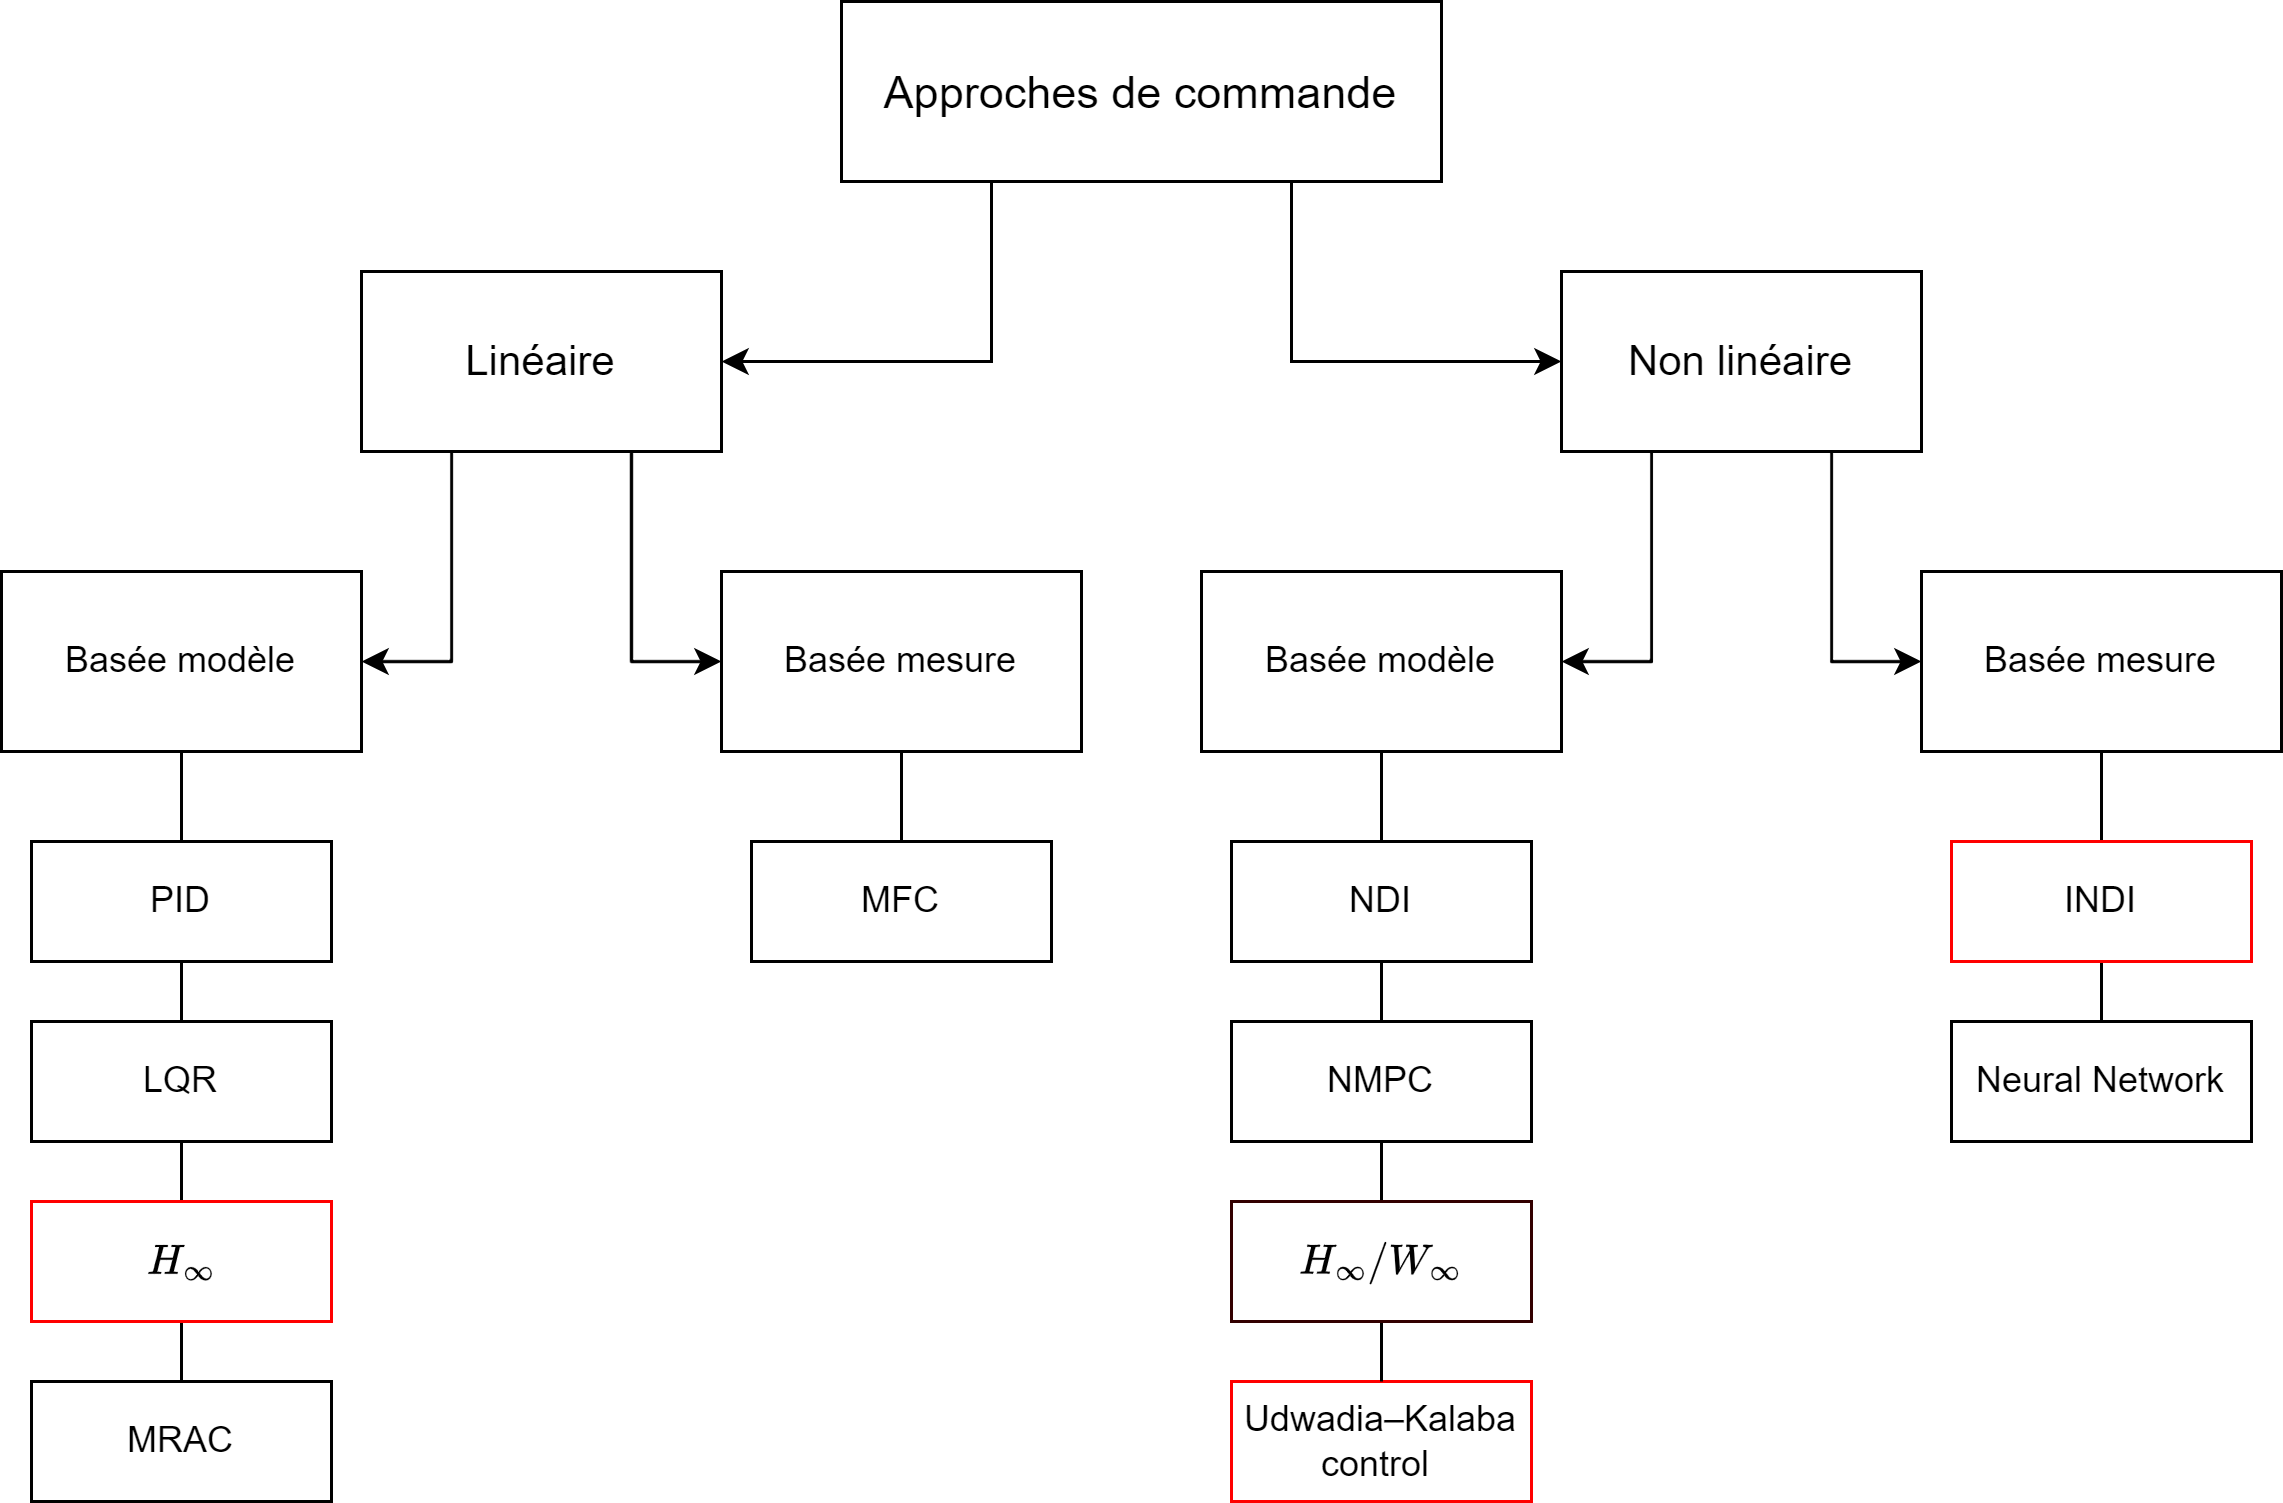
\includegraphics[trim=0cm 0cm 0cm 0cm,clip,width=0.8\columnwidth]{figures/controle_methode.png}}
    \caption{Méthodes de commande utilisées sur les architectures \textit{tailsitters} et \textit{freewings}.}
    \label{fig:methodecmd}
\end{figure}

Faire un schéma avec les méthodes de commande et encadré en rouge nos lois
état de l'art

\subsection*{Contrôleur PID}
Le contrôle Proportionnel Intégral Dérivé (PID) (ou P/PD/PI) est couramment utilisé, car son réglage est intuitif et ne nécessite qu'une connaissance limitée du système. Le contrôle PID donne souvent de très bons résultats et constitue un excellent point de départ pour la conception de contrôleurs plus avancés.

La forme générale d'un contrôleur PID est la suivante :
\begin{align}
    u_{PID}(t) = K_{p} e(t) + K_{i} \int_{0}^{t} e(\tau) \,d\tau + K_{d} \frac{d e(t)}{dt}
\end{align}
\subsection*{Contrôleur LQR}
Les contrôleurs LQR sont un type de contrôle linéaire basée sur les systèmes linéarisés de la forme $\dot{x} = Ax+Bu$. La commande $u$ est
choisie comme :
\begin{align*}
    u = -Kx.
\end{align*}
Ainsi, la matrice de gain K est optimisée pour obtenir de bonnes performances pour le système en boucle fermée par rapport à la fonction de coût
\begin{align*}
    J = \int_{0}^{\infty} x^{\top}(\tau)Q x(\tau) + u^{\top}(\tau)R u(\tau) \,d\tau
\end{align*}
où Q et R sont, respectivement, les matrices de pondération de l'état et des commandes. Bien que le contrôleur LQR présente généralement de bonnes propriétés de robustesse, l'optimalité n'est plus assurée si des erreurs de modélisation et des perturbations sont présentes dans le système. Une discussion détaillée et une comparaison entre le contrôle PID sans modèle et le contrôle LQR basé sur le modèle d'un \textit{tailsitters} est disponible dans \cite{BarthCondomines2018}.
Les auteurs de \cite{Lustosa2017LaP} ont proposé l'approche de séquencement des gains obtenu pour un ensemble de modèle linéaire. Cette architecture de contrôle optimise le gain K en boucle fermée afin de répondre aux exigences de contrôle de la vitesse et de l'attitude définies par l'utilisateur. Grâce à des simulations de vol et à des vols expérimentaux, l'auteur souligne et prouve qu'une seule matrice de gains LQR n'est pas suffisante pour stabiliser le \textit{tailsitter} dans toute son enveloppe de vol, ce qui justifie l'utilisation de méthodes de séquencement des gains.

\subsection*{Contrôleur $H_{\infty}$}
La synthèse $H_{\infty}$ est une méthode qui sert à la conception de commandes optimales, en imposant des contraintes sur la norme $H_{\infty}$ d'un système. En se basant sur une synthèse $H_{\infty}$, les auteurs de \cite{SunYang2009} ont obtenu la stabilisation longitudinale d'un \textit{tiltrotor}. En combinant une synthèse $H_{\infty}$ à une approche de séquencement des gains, les auteurs de \cite{DickesonMix2005, DickesonCifdaloz2006,DickesonMiles2007} ont proposé la stabilisation d'un \textit{tiltwing} sur l'ensemble de son enveloppe de vol. 

\begin{figure}[ht!]
    \centerline{
    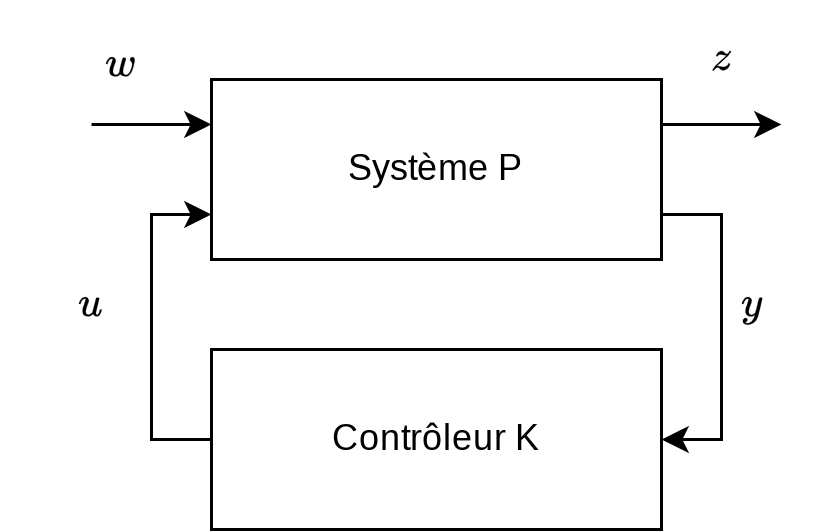
\includegraphics[trim=0cm 0cm 0cm 0cm,clip,width=0.5\columnwidth]{figures/lft.png}}
    \caption{Architecture d'un contrôleur $H_{\infty}$ .}
    \label{fig:schemalft}
\end{figure}

La structure classique d'un contrôleur $H_{\infty}$ est représenté sur la figure \ref{fig:schemalft}. L'objectif est de minimiser l'effet de la perturbation (pire cas) possible $w$ sur la variable de performance $z$ par le biais d'un contrôleur par retour de sortie de la forme $u = K(s) y$. En d'autres termes, K est choisi de telle sorte que $\| F(P, K)\|_{\infty}$  soit minimisé, où $F(P, K)$ est la fonction de transfert de la perturbation $w$ vers le signal d'erreur $z$. 

Nous pouvons aussi citer le travail de \cite{SNYDER2021106621} qui utilise une approche de contrôle $H_{\infty}$ ainsi qu'une représentation du système \textit{Linear Parameter Varying} (LPV). Cette représentation permet d'avoir la dynamique linéaire du drone sur l'ensemble du domaine de vol par interpolation de dynamique parametre par la vitesse totale du drone.
\nomenclature[]{\(LPV\)}{Système linéaire à paramètres variant (\textit{Linear Parameter Varying})}

Enfin, il existe une extension non-linéaire de l'approche approches $H_{\infty}$ en utilisant l'espace de Sobolev pondéré $W_{\infty}$ \cite{cardoso2018nonlinear, CardosoEsteban2019, cardoso2021robust, cardoso2024robust}. Cette méthode s'appuis sur la norme de Sobolev $W_{m,p}$  d'un signal, laquelle est définie par :
\begin{align*}
    \|\boldsymbol{z(t)}\|_{W_{m,p}} = \left( \int_{t_{0}}^{\infty}(\|\boldsymbol{z(t)}\|^{p} + \|\frac{d \boldsymbol{z(t)}}{dt}\|^{p} + ... + \|\frac{d^{m} \boldsymbol{z(t)}}{dt^{m}}\|^{p}) dt \right)^{\frac{1}{p}}.
\end{align*}  

Grâce à la nature de la norme $W_{m,p}$, la variable de coût et ses dérivées temporelles sont prises en compte dans la fonction de coût, ce qui permet d'obtenir des contrôleurs offrant de meilleures performances en régime transitoire et en régime permanent.

\subsection*{Contrôleur non linéaire}

\subsection*{Contrôleur séquencé}
L'approche Diviser et Conquérir permet de passer discrètement d'une loi de contrôle à l'autre, de sorte qu'un seul contrôleur fonctionne à la fois. Un exemple d'un contrôle séquencé hybride de \textit{tailsitters} est donnée dans \cite{Casau2011}.

Contrairement à Diviser et Conquérir, la pondération de contrôle fusionne en continu les commandes de deux contrôleurs, sur la base d'un poids dépendant d'une variable de sélection. Les auteurs de \cite{Liang2016} ont développé deux contrôleurs, un pour le mode VTOL et un second pour la croisière. Ils fonctionnent simultanément et la commande globale est calculée comme  :
\begin{align*}
    u(\Delta t) = (1 - \frac{\Delta t}{T_[T]})u_{VTOL}(\Delta t) + \frac{\Delta t}{T_[T]}u_{cruise}(\Delta t).
\end{align*}
Cet exemple est une transition entre le mode vol stationnaire et le mode croisière. Dans ce cas, $T_[T]$ est le paramètre de durée de la transition et $\Delta t$ est le temps écoulé depuis le début de la manœuvre.

\subsection*{Contrôleur adaptatif}
\nomenclature[]{\(MRAC\)}{Commande adaptative à référence de modèle (\textit{ Model Reference Adaptive Control})}
La commande adaptative à référence de modèle (MRAC) utilise un modèle de référence avec les performances de suivi souhaitées et adapte le contrôleur en fonction de la différence entre le modèle réel et le modèle de référence.

\begin{figure}[ht!]
    \centerline{
    \includegraphics[trim=0cm 0cm 0cm 0cm,clip,width=0.5\columnwidth]{figures/Mrac.png}}
    \caption{Architecture d'un contrôleur MRAC .}
    \label{fig:schemaMRAC}
\end{figure}


\section{Technologies et réalisations}
\todo{Quelques lignes sur les contributions dans paparazzi et am32}
Faire un schéma des composants avec nos contributions

\todo{Conclusion }